\newpage
\section{Versuchsdurchführung}
\label{sec:durchfuerung}
%Ausführliche Beschreibung der eigenen Versuchsdurchführung in Sätzen.
%- Einbindung der eigenen Beobachtungen und der Notizen aus dem
%Beobachtungsprotokoll.
%- Benennung der ggf. während des Versuches aufgetretenen Schwierigkeiten,
%Probleme oder unerwarteten Phänomene.

\begin{figure}[h!]
	\centering
	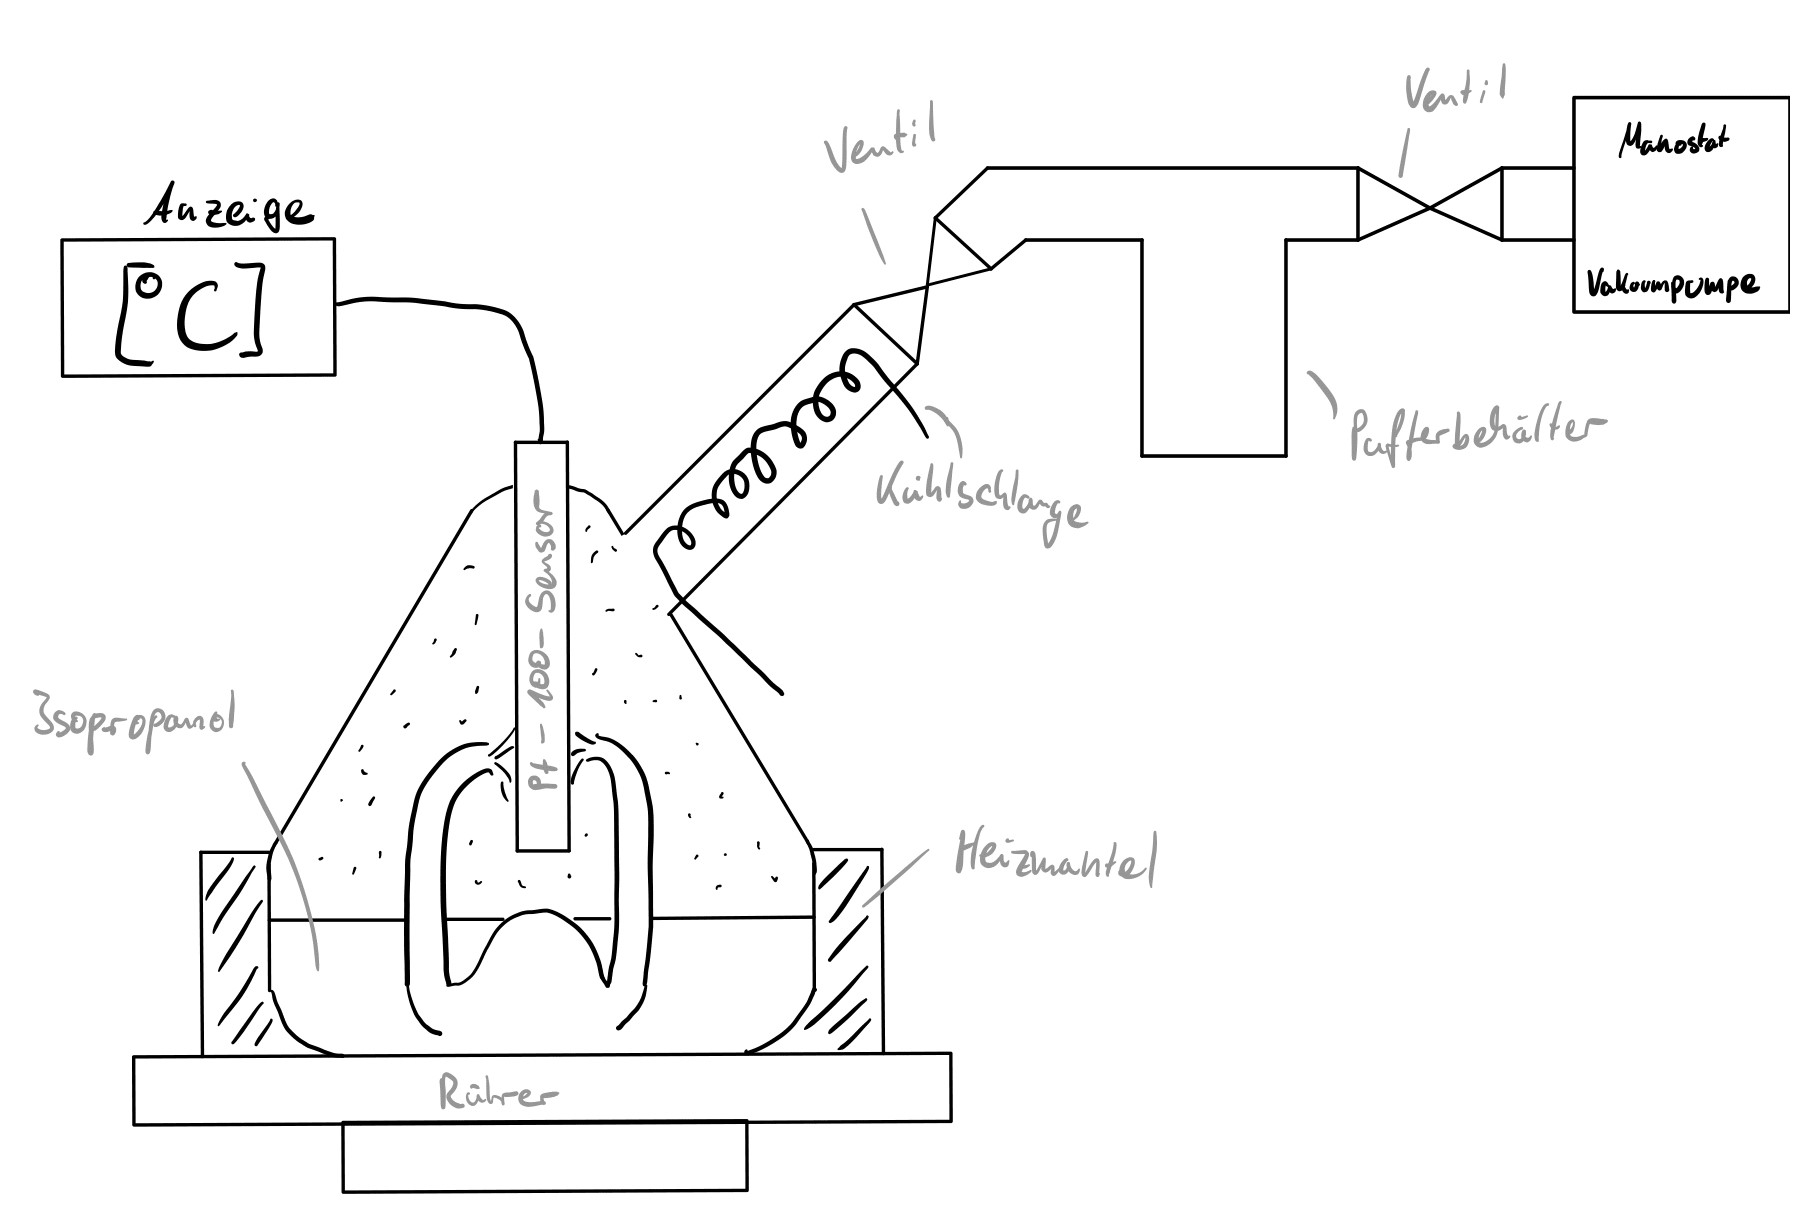
\includegraphics[width=0.8\textwidth]{aufbau}
	\caption{Skizze des Versuchsaufbaus}
	\label{fig:aufbau}
\end{figure}
\FloatBarrier
%Ende

Für den durchgeführten Versuch wurde ein Versuchsaufbau gewählt, ähnlich der Skizze in Abb. \ref{fig:aufbau}. \\
Im Versuch erfolgte im ersten Schritt die Messung des Umgebungsdruckes. Hierfür wurde das Manostat eingeschaltet und das erste Ventil zur Umgebung hin geöffnet. \linebreak
Im zweiten Schritt erfolgen die fokussierte Druck-und Temperaturmessungen des Versuches. Hierfür wird am Druckregler der gewünschte Druck eingestellt und über beide Hähne eine Verbindung zum Probenraum hergestellt. Im Probenraum findet sich in diesem Versuch reines Isopropanol. Nach Einstellung des Drucks erfolgt das Beheizen mittels Heizband, welches über einen Trafo manuell geregelt wird. Im Praktikum wird eine Spannung \SI{220}{\volt} empfohlen. 
Beginnt die Probe zu Sieden ist darauf zu achten, dass das Thermometer für die Temperaturmessung sowohl mit der Gas- als auch der siedenden Flüssigphase in Kontakt steht. Verwendet wird an dieser Stelle ein Pt-100 Widerstandsthermometer. Weist der Verlauf auf der Computeranzeige, für die Temperaturmessung, einen konstanten Verlauf an, so kann die Messung der Siedetemperatur für den nächsten Druck erfolgen.
Der Trafo für das Heizband wird dafür auf \SI{0}{\volt} eingestellt und die entsprechenden Hähne zum Probenraum geschlossen. \linebreak
Sind die vorangegangenen Schritte absolviert, kann mit dem Einstellen eines weiteren Drucks begonnen werden. Wichtig für das folgende Vorgehen ist, dass der Hahn zum Probenraum hin nur langsam geöffnet wird, um zu starke Siedeverzugseffekte zu vermeiden.